\section{RQ1: Reproduction of the Paper}
\label{sec:rq1}

The three models of~\cite{severson2019} were rebuilt on F1--F3 with the
protocol of Section~\ref{sec:methods}. The variance model is
$\log_{10}(\text{life}) = 1.346 - 0.396\,\log_{10}\mathrm{Var}(\dq)$. For
the discharge and full models, cross-validation chose an almost ridge-like
penalty ($\rho=0.1$; $\alpha=0.022$ and $0.039$), keeping 6 of 6 and 7 of 9
features.

\begin{table}[!htb]
\centering
\caption{Reproduction of Table~1 of~\cite{severson2019}: ours (paper).
Prim.\ excl.: primary set without \texttt{b2c1}.}
\label{tab:repro}
\small
\setlength{\tabcolsep}{3pt}
\begin{tabular}{@{}lcccc@{}}
\toprule
Model & Train & Primary & Prim.\ excl. & Secondary \\
\midrule
\multicolumn{5}{@{}l}{\textit{RMSE (cycles)}} \\
Constant  & 327 (327) & 401 (401) & 399 (399) & 511 (511) \\
F1 Variance & 104 (103) & 138 (138) & 138 (138) & 196 (196) \\
F2 Discharge & 69 (76) & 90 (91) & 85 (86) & 167 (173) \\
F3 Full & 67 (51) & 125 (118) & 122 (100) & 220 (214) \\
\midrule
\multicolumn{5}{@{}l}{\textit{Mean absolute percentage error (\%)}} \\
Constant  & 29.6 (29.6) & 35.0 (34.9) & 28.2 (28.2) & 36.1 (36.1) \\
F1 Variance & 14.1 (14.1) & 14.7 (14.7) & 13.2 (13.2) & 11.4 (11.4) \\
F2 Discharge & 9.2 (9.8) & 12.6 (13.0) & 9.4 (10.1) & 9.9 (8.6) \\
F3 Full & 6.8 (5.6) & 11.0 (14.1) & 8.0 (7.5) & 11.2 (10.7) \\
\bottomrule
\end{tabular}
\end{table}

\textbf{Results} (Table~\ref{tab:repro}). The constant and variance models match exactly on the test sets. The
discharge model is within 1--6 cycles and the full model within 7 cycles on
both full test sets; the full model's gap is larger on the training set (67 vs.\ 51) and on
the primary set without \texttt{b2c1} (122 vs.\ 100). These gaps are comparable to our own spread over 10 random seeds
(full model: primary 117--128, secondary 218--222 cycles) and are expected
from the paper's different software and sampling. The ranking is the
same, including the paper's key observation that the full model is
\emph{worse} than the discharge model on the secondary set, and the
full-model coefficients agree in sign with the paper's wherever both are
non-zero.

\begin{figure}[!htb]
  \centering
  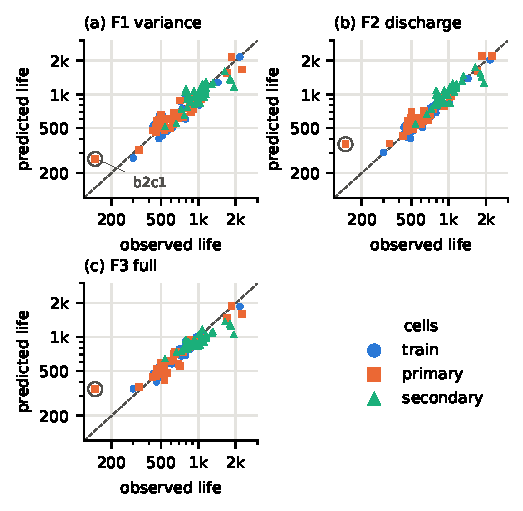
\includegraphics[width=\columnwidth]{fig_rq1_parity}
  \caption{Predicted vs.\ observed cycle life of the three reproduced models
  (log axes; cf.\ Fig.~3 of~\cite{severson2019}). Circled: the anomalous
  cell \texttt{b2c1}.}
  \label{fig:parity}
\end{figure}

\textbf{Where the errors are.} Few training cells live beyond 1500 cycles,
so all three models under-predict the longest-lived cells
(Fig.~\ref{fig:parity}). The longest, \texttt{b1c2} (2237 cycles), is
predicted at 1594 by the full model and alone causes 63\,\% of its squared
error on the primary set. \texttt{b2c1} (148 cycles) is predicted at
266--360; its early failure is not visible in the first 100 cycles.
Within b2 the discharge model is no better than the variance model (MAPE
18.0 vs.\ 17.9\,\% on the primary b2 cells): the skewness and kurtosis of
$\Delta Q$ change sign between b1 and b2 (Table~\ref{tab:featsets}) and get
small weights, so its gain over F1 comes from b1.

\textbf{A data fault.} The first full-model fit predicted 0 cycles for
\texttt{b1c18} (observed 691). In its cycles 2--53 the resistance logger
repeats 19.886\,m$\Omega$ 52 times, and every record contains a time-stamp
jump of 35--67\,h that inflates the temperature integral to 372 standard
deviations above the training mean. Rules C6 and C7
(Table~\ref{tab:cleaning}) fix both, and the prediction becomes 578 cycles.

\textbf{Answer to RQ1.} Yes: the published results are reproduced, exactly
for the variance model and within 7 cycles on the test sets for the others,
with the same ranking.
